\section{Durchführung}
\label{sec:Durchführung}
Das hier verwendete Diffraktometer besteht aus einer Röntgenröhre auf der einen und einem Empfänger für Röntgenstrahlung auf der anderen Seite. Mittig zwischen ihnen ist ein Tisch für die Probe platziert. Zur Steuerung des Versuchsaufbau wird das Programm XRD-Commander verwendet.

\subsection{Justage}
Da die Probe, welche hier ein mit einer dünnen Polystyrolschicht überzogener Silizium-Wafer ist, nach dem Einbringen in den Versuchsaufbau noch nicht die richtige Ausrichtung hat, muss der Aufbau zunächst justiert werden. Ziel der Justage ist es, die Probe genau mittig zwischen Sender und Empfänger zu platzieren, sodass die gesamte Strahlung der Röntgenröhre auf die Probe trifft. Außerdem muss die Nullposition für Sender und Empfänger so justiert werden, dass die Probe bei einem Glanzwinkel von null genau parallel zum Strahl steht.\\
\\
Im ersten Schritt der Justage wird daher ein Detektorscan durchgeführt. Bei diesem wird die Röntgenröhre direkt auf den Detektor gerichtet. Der Detektor wird im Winkel variiert und durch den Strahl gefahren. Das Maximum dieser Gauß-verteilten Messung wird dann als neue Null-Position eingestellt.\\
\\
Als Nächstes wird die Probe in den Strahl eingebracht. Da zuvor die der gesamte Strahl den Detektor traf, lässt sich durch Hochfahren Bewegen der Probe im Strahl der Punkt in z-Richtung bestimmen, bei welchem ungefähr der halbe Strahl abgeschattet ist. Dies wird mithilfe eines \textit{Z-Scan}s bewerkstelligt. Dieser verschiebt die Probe wie in \autoref{fig:z} gezeigt in z-Richtung. Auf diesen Punkt wird die Probe gesetzt. Da die Feinjustage später kommt, reicht hier ein ungefährer Wert.\\
\\
\begin{figure}
    \centering
    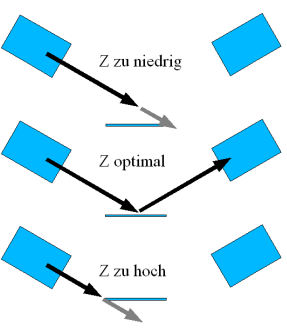
\includegraphics[width=0.5\textwidth]{figures/z.png}
    \caption{Veranschaulichung der Funktionsweise des z-Scans.}
    \label{fig:z}
\end{figure}
Der folgende Scan dient dazu, den Einfallswinkel gleich dessen Ausfallswinkel zu setzen. Dazu werden Röntgenröhre und Detektor um die Probe rotiert, ohne ihre relative Ausrichtung zu einander zu ändern. Dieser Scan heißt \textit{Rocking-Scan} (engl. \textit{to rock}: Schaukeln). Dessen Funktionsweise ist in \autoref{fig:rocking} veranschaulicht. Da dieser Scan den Strahl einmal mit der dem Emitter und einmal mit der dem Detektor zugewandten Kante der Probe verdeckt, liefert er Aufschluss über die Positionierung der Probe entlang des Strahls. Das Ergebnis dieses Scans sollte ein gleichseitiges Dreieck sein. Ist dies nicht der Fall, muss die Probe entlang des Strahls verschoben werden, bis ihre Ausrichtung passt, damit später auch wirklich der gesamte Strahl die Probe trifft. Nach dieser Justage wird das Maximum des Rockingscans als neue Nulllage des Emitter-Detektor-Paars gewählt, damit der Strahl nun genau parallel zur Oberfläche der Probe steht.\\
\\
\begin{figure}
    \centering
    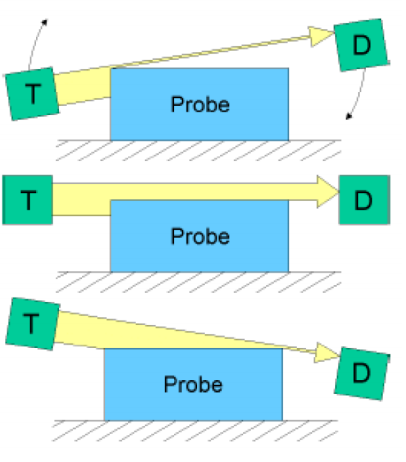
\includegraphics[width=0.5\textwidth]{figures/rocking.png}
    \caption{Veranschaulichung der Drehbewegung und Funktionsweise des Rocking-Scans.}
    \label{fig:rocking}
\end{figure}
Im Anschluss wird ein weiterer Z-Scan durchgeführt, um eine präzisere halbe Abschattung des Strahls zu erreichen.\\
\\
Ein anschließender Rocking-Scan, mit einem Glanzwinkel von $0.15^\circ$ verfeinert die Parallelität der Probe zum Strahl.\\
\\
Zum Schluss wird für den selben Glanzwinkel ein letzter Z-Scan durchgeführt und die Probe wieder auf die halbe Abschattung gesetzt. Dieser sorgt dafür, dass der Strahl genau mittig auf die Probe trifft.

\subsection{Reflektivitätsmessung}
Die eigentliche Messung dient zur Bestimmung der Reflektivität. Um diese zu bestimmen, muss wie zuvor beschrieben ein Winkelbereich abgefahren werden. Dabei werden Emitter und Detektor gleichzeitig immer um den selben Glanzwinkel verschoben, um so die Intensität des reflektierten Strahls unter verschiedenen Winkel zu messen. Hier wurde ein Winkelintervall von $[0^\circ,2.5^\circ]$ gewählt, mit einer Schrittweite von $0.005^\circ$.\\
\\
Um den Untergrund der Reflektivitätsmessung zu bestimmen, wird der selbe Scan erneut durchgeführt, allerdings mit um $0.1^\circ$ verschobenem Detektor, was als \textit{diffuser Scan} bezeichnet wird. 
\cite{Anleitung44}